\section{Generalized Morton Layouts}

\label{sec:bijections}

\begin{figure}
\begin{subfigure}{0.25\columnwidth}\centering\curve{0,0,0,1,1,1}\vspace{-1.5mm}\caption{[0,0,0,1,1,1]}\vspace{1.5mm}\label{fig:layouts8x8:000111}\end{subfigure}\hfill
\begin{subfigure}{0.25\columnwidth}\centering\curve{0,0,1,0,1,1}\vspace{-1.5mm}\caption{[0,0,1,0,1,1]}\vspace{1.5mm}\end{subfigure}\hfill
\begin{subfigure}{0.25\columnwidth}\centering\curve{0,0,1,1,0,1}\vspace{-1.5mm}\caption{[0,0,1,1,0,1]}\vspace{1.5mm}\end{subfigure}\hfill
\begin{subfigure}{0.25\columnwidth}\centering\curve{0,0,1,1,1,0}\vspace{-1.5mm}\caption{[0,0,1,1,1,0]}\vspace{1.5mm}\end{subfigure}\\
\begin{subfigure}{0.25\columnwidth}\centering\curve{0,1,0,0,1,1}\vspace{-1.5mm}\caption{[0,1,0,0,1,1]}\vspace{1.5mm}\end{subfigure}\hfill
\begin{subfigure}{0.25\columnwidth}\centering\curve{0,1,0,1,0,1}\vspace{-1.5mm}\caption{[0,1,0,1,0,1]}\vspace{1.5mm}\label{fig:layouts8x8:010101}\end{subfigure}\hfill
\begin{subfigure}{0.25\columnwidth}\centering\curve{0,1,0,1,1,0}\vspace{-1.5mm}\caption{[0,1,0,1,1,0]}\vspace{1.5mm}\end{subfigure}\hfill
\begin{subfigure}{0.25\columnwidth}\centering\curve{0,1,1,0,0,1}\vspace{-1.5mm}\caption{[0,1,1,0,0,1]}\vspace{1.5mm}\end{subfigure}\\
\begin{subfigure}{0.25\columnwidth}\centering\curve{0,1,1,0,1,0}\vspace{-1.5mm}\caption{[0,1,1,0,1,0]}\vspace{1.5mm}\end{subfigure}\hfill
\begin{subfigure}{0.25\columnwidth}\centering\curve{0,1,1,1,0,0}\vspace{-1.5mm}\caption{[0,1,1,1,0,0]}\vspace{1.5mm}\end{subfigure}\hfill
\begin{subfigure}{0.25\columnwidth}\centering\curve{1,0,0,0,1,1}\vspace{-1.5mm}\caption{[1,0,0,0,1,1]}\vspace{1.5mm}\end{subfigure}\hfill
\begin{subfigure}{0.25\columnwidth}\centering\curve{1,0,0,1,0,1}\vspace{-1.5mm}\caption{[1,0,0,1,0,1]}\vspace{1.5mm}\end{subfigure}\\
\begin{subfigure}{0.25\columnwidth}\centering\curve{1,0,0,1,1,0}\vspace{-1.5mm}\caption{[1,0,0,1,1,0]}\vspace{1.5mm}\label{fig:layouts8x8:100110}\end{subfigure}\hfill
\begin{subfigure}{0.25\columnwidth}\centering\curve{1,0,1,0,0,1}\vspace{-1.5mm}\caption{[1,0,1,0,0,1]}\vspace{1.5mm}\end{subfigure}\hfill
\begin{subfigure}{0.25\columnwidth}\centering\curve{1,0,1,0,1,0}\vspace{-1.5mm}\caption{[1,0,1,0,1,0]}\vspace{1.5mm}\end{subfigure}\hfill
\begin{subfigure}{0.25\columnwidth}\centering\curve{1,0,1,1,0,0}\vspace{-1.5mm}\caption{[1,0,1,1,0,0]}\vspace{1.5mm}\end{subfigure}\\
\begin{subfigure}{0.25\columnwidth}\centering\curve{1,1,0,0,0,1}\vspace{-1.5mm}\caption{[1,1,0,0,0,1]}\vspace{1.5mm}\end{subfigure}\hfill
\begin{subfigure}{0.25\columnwidth}\centering\curve{1,1,0,0,1,0}\vspace{-1.5mm}\caption{[1,1,0,0,1,0]}\vspace{1.5mm}\end{subfigure}\hfill
\begin{subfigure}{0.25\columnwidth}\centering\curve{1,1,0,1,0,0}\vspace{-1.5mm}\caption{[1,1,0,1,0,0]}\vspace{1.5mm}\end{subfigure}\hfill
\begin{subfigure}{0.25\columnwidth}\centering\curve{1,1,1,0,0,0}\vspace{-1.5mm}\caption{[1,1,1,0,0,0]}\vspace{1.5mm}\label{fig:layouts8x8:111000}\end{subfigure}
\caption{All 20 layouts for $8\times 8$ arrays generated by the family of indexing schemes described in \cref{sec:bijections}. Note that \cref{fig:layouts8x8:000111} corresponds to a row-major layout, while \cref{fig:layouts8x8:111000} corresponds to a column-major layout.}
\label{fig:layouts8x8}
\end{figure}

The Morton layout functions by interleaving the bits of the input indices in a fixed pattern: bits are drawn from each of the inputs in a round-robin manner. In this section, we generalize this idea, allowing bits to be interleaved in arbitrary order. This gives rise to more specialized layouts with different structure and, as a result, different extra-functional properties~\cite{doi:10.1177/1094342017725568,doi:10.1080/17445760902758560,10.1145/1274971.1274989}. \cref{fig:layouts8x8} shows all 20 layouts that are given by different bit interleaving orders for an $8 \times 8$ array. As with the standard Morton layout, the generalized Morton layout can be applied to any number of dimensions. As an example, the following three-dimensional layout selects two bits from the second index, one bit from the third index, then two bits from the first index, etc.:

\begin{equation}
\arraycolsep=1pt
\label{ex:permute:4}
f({\color{Palette1}011}_2, {\color{Palette2}101}_2, {\color{Palette3}100}_2) = \begin{array}{r r}&{\color{gray}0}{\color{Palette1}0}{\color{gray}00}{\color{Palette1}1}{\color{Palette1}1}{\color{gray}000}_2\\\vee&{\color{gray}000}{\color{Palette2}1}{\color{gray}000}{\color{Palette2}01}_2\\&{\color{Palette3}1}{\color{gray}0}{\color{Palette3}0}{\color{gray}000}{\color{Palette3}0}{\color{gray}00}_2\\\hline&{\color{Palette3}1}{\color{Palette1}0}{\color{Palette3}0}{\color{Palette2}1}{\color{Palette1}11}{\color{Palette3}0}{\color{Palette2}01}_2\end{array} = 313_{10}
\end{equation}

Our goal is to find Morton-like layouts i.e., bit-interleaving patterns, that improve application performance through an increase in cache efficacy. In this section, we will show that the design space for such layouts is very large, motivating the use of genetic algorithms. This necessitates a chromosomal representation of layouts, which we also present in this section. In addition, we describe how the canonical layouts can be described using the same representation, and we delve into practical considerations such as the computational cost of computing indices and support for same-instruction multiple-data (SIMD) processing.

\subsection{Enumerating Layouts}

\label{sec:bijections:enumerating}

We can characterize Morton-like layouts by the bit scattering pattern applied to each of the inputs (e.g., for \cref{ex:permute:4}, the first index is scattered to the fourth, fifth, and eighth bits). However, such a characterization is unsound in the sense that is allows us to describe invalid layouts: if two bits from any of the input indices are mapped onto the same bit in the output, the bitwise disjunction becomes an information-destroying operation and the layout becomes non-injective---that is, it would cause multiple multi-dimensional indices to map onto the same location in memory, making the layout unusable.

We can instead characterize layouts in a manner that is both complete and sound by enumerating the \emph{source} of each bit in the output index. In the remainder of this work we shall denote array layouts using sequences of the form $[i_0, \ldots, i_{n-1}]$, indicating the source indices in order of increasing bit significance: the least significant bit in the output index is drawn from the $i_0$th input index, the second-least significant bit is drawn from the $i_1$th input, and the most significant bit is drawn from the $i_{n-1}$th input. Note that each input bit must be used once and only once: whenever a bit is to be drawn from a given input index, we implicitly use the least significant bit for that input which has not yet been consumed. For the layout shown in \cref{ex:permute:4}, the two least significant bits are drawn from the second input, the third-least significant bit is drawn from the third input, and so forth: the resulting array layout is denoted using the sequence $[1,1,2,0,0,1,2,0,2]$. 

The aforementioned characterization of multi-dimensional layouts gives rise to families of layouts. The family of layouts over $n$ inputs, where each input has $b_0,\ldots,b_{n-1}$ bits, is isomorphic to the set of permutations of the multiset $S = \{0:b_0,\ldots,n-1:b_{n-1}\}$. We denote this set of permutations as $\mathfrak{S}(S)$. For convenience, we obviate the intermediate multiset such that $\mathfrak{S}'(b_0,\ldots,b_{n-1}) = \mathfrak{S}(\{0:b_0,\ldots,n-1:b_{n-1}\})$. We can then determine the total number of possible layouts as the number of multiset permutations of $\mathfrak{S}'$~\cite[p.~42]{brualdi1977introductory}:

\begin{equation}
\label{eq:permutation_set_size}
|\mathfrak{S}'(b_0, \ldots, b_{n-1})| = \binom{\sum_{i = 0}^{n-1} b_i}{b_0,\ldots,b_{n-1}} = \frac{\big(\sum_{i = 0}^{n-1} b_i \big)!}{\prod_{i = 0}^{n-1} (b_i!)}    
\end{equation}

\subsection{Including Canonical Layouts}

\label{sec:bijections:canonical}

It is worth noting that canonical layouts over arrays for which the size in each dimension is a power of two are, in fact, members of the family of Morton-like layouts. In order to sketch an informal argument for this, we recall that the indexing function for an $n$-dimensional canonical layout given array sizes $N_0, \ldots, N_{n-1}$ is defined as in \cref{eq:lexicographic}. If we assume that all sizes are powers of two, then the product of these sizes is guaranteed to be itself a power of two. Because multiplication by powers of two can be interpreted as a left-ward shift, the canonical layouts shift each input index $x_0, \ldots, x_n$ to a specific location in the binary expansion of the output index. Furthermore, because we assume $\forall i : x_i < N_i$, each bit in the output is determined by exactly one of the input indices; this allows us to interpret the summation as a series of bit-wise disjunctions, exactly like the definition of our Morton-like layouts. In general, a mode-0-major canonical layout of a $2^{b_0} \times \ldots \times 2^{b_{n-1}}$ array can be characterized---in the the scheme defined in \cref{sec:bijections:enumerating}---by contiguous subsequences of bits, each drawn from the same index i.e., a sequence of the following form:

\begin{equation}
\label{eq:cacnonical_repr}
[\underbrace{0,\ldots,0}_{b_0\text{ times}}, \underbrace{1,\ldots,1}_{b_1\text{ times}}, \ldots, \underbrace{n-1,\ldots,n-1}_{b_{n-1}\text{ times}}]    
\end{equation}

Canonical layouts with different major axes can be constructed by changing the order of the contiguous subsequences. The fact that the canonical layouts are members of the Morton-like family of array layouts allows us to evaluate the performance of these layouts in the exact same framework as the rest of the Morton-like layouts, and we will exploit this in \cref{sec:experiments}. %Indeed, we can compare canonical layouts and Morton-layout with the exact same code (even at the assembly level) which ensures that we can evaluate the performance of these layouts in the fairest possible way.

\subsection{Hardware-Accelerated Indexing}

\label{sec:bijections:accel}

It is tempting to extend the aforementioned ideas to even more exotic indexing functions, like the Hilbert array layout~\cite{hilbert1891ueber,10.1145/3555353,10.1007/978-3-642-25100-9_73}. The computational cost of many such functions renders them impractical, however: if the cost of computing memory addresses is too large, any performance gained by improving the cache-friendliness of a program will be negated. The Morton-like layouts we consider in this work allow efficient index calculations on modern commodity hardware, which we demonstrate in this section.

Under canonical array layouts, indices are calculated either iteratively through repeated addition and multiplication, or in parallel through parallel multiplication followed by reduction through addition. In $n$-dimensional cases both approaches require $n-1$ additions and $n-1$ multiplications, operations which can be efficiently performed on virtually all processors. Specifically, the Intel Haswell and AMD Zen 3 microarchitectures---on which we focus in this work---can perform 64-bit register addition (\texttt{ADD r64 r64}) with a latency 1 cycle and a reciprocal throughput of 0.25 cycles, while they can execute multiplication (\texttt{IMUL r64 r64}) with a latency of 3 cycles and a reciprocal throughput of 1 cycle~\cite{10.1145/3297858.3304062}.

Our bit-interleaving array layouts rely, in $n$-dimensional cases, on $n-1$ bitwise disjunctions and $n$ bit-scatter operations. Such disjunctions (\texttt{OR r64 r64}) can be performed with a latency of 1 cycle and a reciprocal throughput of 0.25 cycles---the same as the \texttt{ADD} instruction---on both of the aforementioned microarchitectures. We perform the bit-scattering operation using the \emph{parallel bit deposition} (\texttt{PDEP r64 r64 r64}) instruction, which is included in the BMI2 extension to the x86-64 instruction set~\cite{10.1145/3319647.3325833}. The Intel Haswell and AMD Zen 3 microarchitectures both perform bit deposition with a latency of 3 cycles and a reciprocal throughput of 1 cycle, identical to the \texttt{IMUL} instruction. It follows that Morton-like indexing requires---in theory---only a single additional instruction over canonical index calculation.

The hardware extension required to perform bit deposition is widely supported: BMI2 has been included in Intel processors starting with the Haswell microarchitecture (2013)~\cite{6762795}, and in AMD processors starting with the Excavator microarchitecture (2015), albeit in a limited fashion; AMD processors gained full hardware support for these instructions starting with the Zen 3 microarchitecture (2020)~\cite{9718180}\footnote{Pre-Zen 3 processors supported parts of the BMI2 instruction set---the \texttt{PEXT} and \texttt{PDEP} instructions in particular---through emulation in microcode rather than in hardware, making them very slow.}. 

\begin{figure}
    \centering
    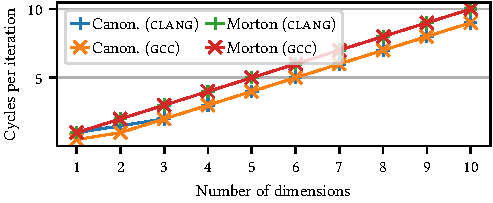
\includegraphics{figures/canon_vs_morton_cycles.pdf}
    \caption{Throughput of a kernel calculating array indices using canonical layouts as well as Morton-like layouts on the Intel Haswell microarchitecture as given by \textsc{OSACA}.}
    \label{fig:canon_vs_morton}
\end{figure}

In order to further evaluate the competitiveness of Morton-like layouts compared to canonical layouts, we analyze implementations of both indexing schemes over a range of dimensionalities as compiled by \textsc{gcc} 12.3 and \textsc{clang} 15.0 using \textsc{OSACA} 0.5.2~\cite{8641578}. All code was compiled using the \texttt{-O2} optimization flag. The results of this analysis are shown in \cref{fig:canon_vs_morton}. Over the range of dimensionalities considered, the canonical layouts are consistently faster i.e., require fewer cycles to compute, than the Morton-like layouts. However, the difference in performance---approximately one cycle---is relatively small and overshadowed by the number of cycled saved due to a reduction in cache misses. Furthermore, we focus primarily on memory-bound applications, in which a small increase in index calculation time is unlikely to affect performance. We conclude, therefore, that Morton-like layouts are competitive with canonical layouts strictly in terms of address computation costs.

\subsection{Support for SIMD}

\label{sec:bijections:SIMD}

An important consideration in the design of array layouts is the ability to vectorize kernels through single-instruction multiple-data (SIMD) operations. Canonical layouts guarantee the contiguity of fibers in the array, which facilitates the (automated) vectorization (e.g., the application of SIMD) of many operations, and this benefit is lost when applying the array layouts discussed in this paper. However, we posit that there remains ample opportunity to accelerate computation on Morton-like arrays using SIMD, and we argue this by distinguishing two classes of computation patterns.

The first class consists of \emph{unstructured} patterns in which data is operated on element-wise without spatial context i.e., without consideration of nearby elements; a prominent example of such an operation is matrix \emph{addition}. In such applications, SIMD can be trivially applied to the underlying one-dimensional memory, regardless of the layout of the data: since elements can be added point-wise in any order, doing so in the order in which the data is laid out in memory is both feasible and enables SIMD.

The second class of problems consists of \emph{structured} patterns in which operations must be performed in a specific order. A prime example of such an operation is matrix \emph{multiplication} where the inner product of fibers must be computed. In such cases, it is imperative that fibers can be accessed in contiguous blocks. The size of these blocks depends on the vectorization technology used as well as the size of the data type: in the x86 instruction set, SSE vectorisation requires two consecutive double-precision numbers or four consecutive single-precision numbers~\cite{intelx86}; the much wider ARM SVE instruction set extension~\cite{7924233} may require up to thirty-two consecutive double-precision numbers or sixty-four single-precision numbers.

In order to facilitate vectorization for structured patterns of computation, we can impose certain constraints on the array layouts we consider. Indeed, if the $n$ least-significant bits of an interleaving pattern are all drawn from the $m$th input index, then the layout guarantees that the mode-$m$ fibers in the array are contiguous in blocks of $2^n$ elements. This requirement can be incorporated into the selection of array layouts; for example, we can enable efficient AVX2 vectorisation (with a vector width of 256 bits) using single-precision (32-bit) floating point numbers by ensuring that the three least significant bits in an array layout are drawn from the same source. In other words, we can easily constrain our search space to include only array layouts with properties that favor vectorization, and we believe that doing so will enable SIMD-accelerated computation arrays laid out in Morton-like orders.
